\documentclass[12pt]{article}
% Commands
\newcommand{\code}[1]{\texttt{#1}}
% Packages
\usepackage[dutch]{babel}
\usepackage{graphics}
\usepackage{graphicx}
\usepackage[rightcaption]{sidecap}
\usepackage{enumerate}
\usepackage{multirow}
\usepackage{array}
\usepackage{listings}
\usepackage{color}
\usepackage{mathtools}
\usepackage[a4]{geometry}
% Listing color
\definecolor{dkgreen}{rgb}{0,0.6,0}
\definecolor{gray}{rgb}{0.5,0.5,0.5}
\definecolor{mauve}{rgb}{0.58,0,0.82}
\lstset{frame=tb,
	language=C++,
	aboveskip=3mm,
	belowskip=3mm,
	showstringspaces=false,
	columns=flexible,
	basicstyle={\small\ttfamily},
	numbers=none,
	numberstyle=\tiny\color{gray},
	keywordstyle=\color{blue},
	commentstyle=\color{dkgreen},
	stringstyle=\color{mauve},
	breaklines=true,
	breakatwhitespace=true,
	tabsize=3}
%Path
\graphicspath{ {Images/} }

\begin{document}
	\begin{titlepage}
		\newcommand{\HRule}{\rule{\linewidth}{0.5mm}} 
		\center
		\textsc{\LARGE Hogeschool Utrecht}\\[1.5cm]
		
\includegraphics[scale=.25]{hu-logo}\\ [1cm] % Afbeelding
		\textsc{\Large Group Project}\\[0.5cm] % Cursus naam
		\textsc{\large TICT-V1GP-15}\\[0.5cm] % Cursus code
		\HRule \\[0.4cm]
		{ \huge Het besturingsalgoritme} \\[0.2cm] % Titel
		\HRule \\[1.5cm]
		\begin{minipage}{0.4\textwidth}
			\begin{flushleft} \large
				\center
				\large \emph{Deelnemers:}\\
				Nick \textsc{Snel}\\
				Ramon \textsc{van Bemmel}\\
				Nathan \textsc{Hoekstra}\\
				Cris \textsc{van der Nolle}\\
				Marc \textsc{Dirven}
			\end{flushleft}
		\end{minipage}\\[1cm]
		\Large \emph{Docent:}\\
		Adrie \textsc{Doesburg}\\[.5cm]
		April 13, 2018
	\end{titlepage}
\newpage
	\renewcommand{\contentsname}{Inhoudsopgave} % Assign a new name to ToC
	\tableofcontents
	
\newpage

\section{Inleiding}
	In dit document wordt ingegaan op het door ons ontwikkelde algoritme. Onze robot (gebouwd op LEGO mindstorms) wordt bestuurd door een programma dat draait op een Raspberry Pi en input geeft aan de robot via een BrickPi shield.\\
	De bedoeling van de robot is dat hij volledig autonoom een zwarte lijn volgt op een wit veld. Hij moet dus ook bochten kunnen nemen, objecten kunnen ontwijken en de lijn terug kunnen vinden.\\
	De BrickPi dient voor ons als interface met sensoren en motoren op de robot. De robot zelf is een Lego Mindstorms robot, maar i.p.v. de meegeleverde computer van mindstorms gebruiken we dus bovengenoemde configuratie van Raspberry Pi plus een BrickPi shield en C++ code. Op het BrickPi shield zitten MMJ aansluitingen om via een serieel protocol met de motoren en sensoren te kunnen communiceren.
\newpage

\section{Probleemstelling}
	Het algoritme kan twee parcours volgen. We beschrijven ze hieronder in stapjes:
	\begin{itemize}
		\item \textbf{Parcours 1}:
		\begin{itemize}
			\item Een lijn kan zien door middel van een zwart-wit contrast.
			\item Op een lijn kan blijven door zijn rijrichting aan te passen.
			\item Bij een bocht kan afslaan.
			\item Obstakels op de lijn kan ontwijken.
			\item Zijn weg terug kan vinden naar de lijn.
		\end{itemize}
		\item \textbf{Matrix}:
		\begin{itemize}
			\item Kan navigeren door een grid.
			\item Herkennen van kruispunten.
			\item Het volgen van een lijn.
			\item In staat zijn, zijn route aan te kunnen passen bij een obstakel.
		\end{itemize}
	\end{itemize}
\newpage
\section{Aanpak}
	In dit hoofdstuk zullen we aan de hand van een aantal diagrammen het ontwerp omschrijven.
	\subsection{De Robot}
		De robot is net als alle andere robots gebouwd in Lego Mindstorms. Zie hieronder voor onze robot. Hij heet "Tesla Model S".
		\begin{center}
			\begin{SCfigure}[0][h]
				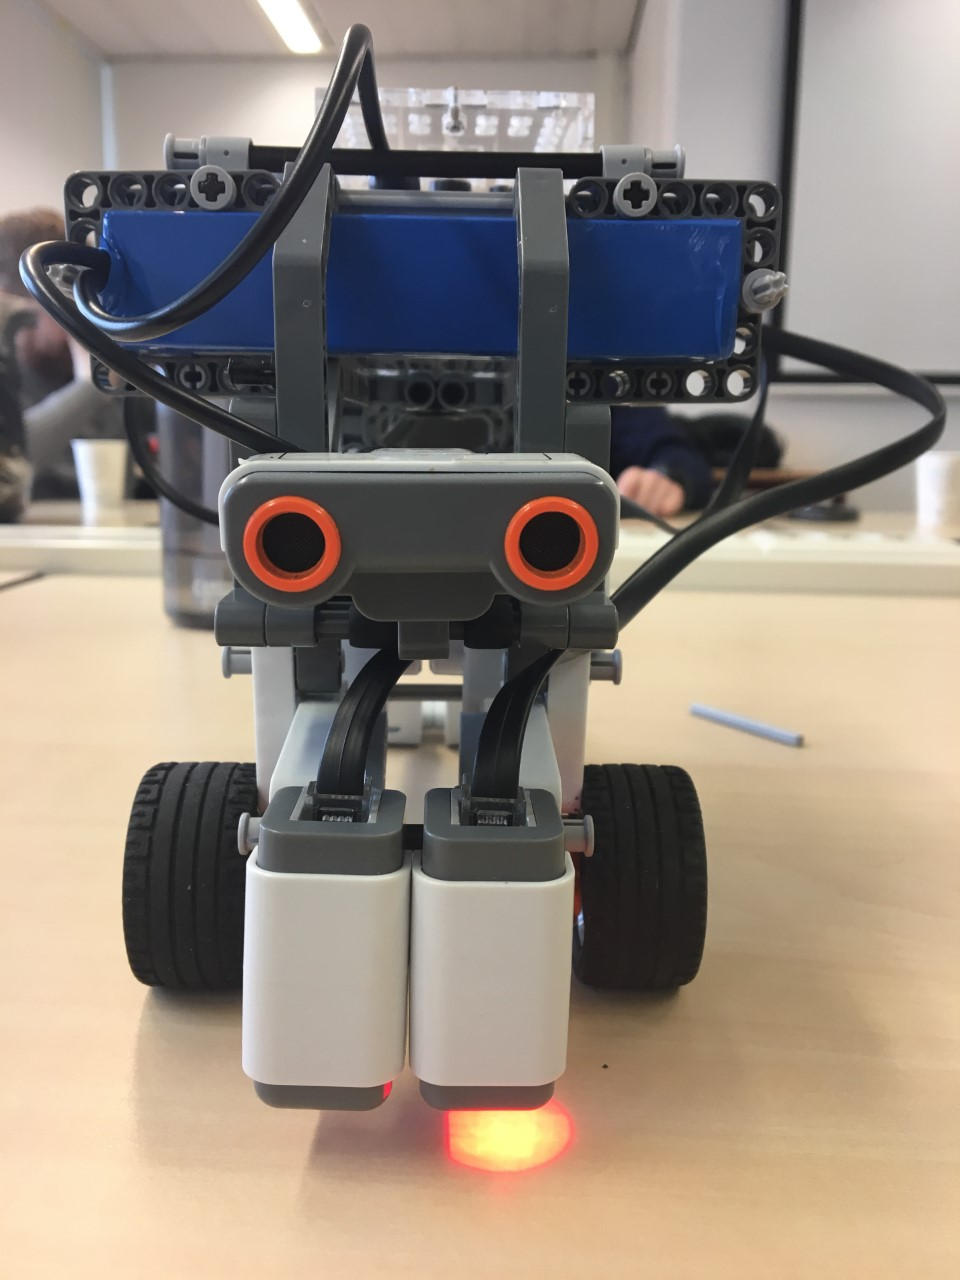
\includegraphics[scale=0.3]{TeslaModelS}	
				\caption{"Model S"}
			\end{SCfigure}
		\end{center}
		Hierbij is de rechter sensor (t.o.v. de rijrichting) de lichtsensor en de linker sensor de kleurensensor. De brede lange sensor aan de bovenkant met de twee oogjes is de ultrasoonsensor.
		\subsection{Use Case Diagram}
			Zie onderstaand figuur voor de Use Case Diagram.
		\begin{center}
			\begin{SCfigure}[0.25][h]
				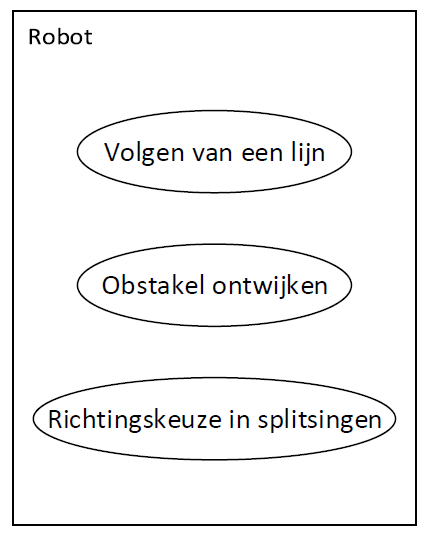
\includegraphics[scale=.7]{UseCase}
				\caption{In deze figuur is te zien welke activiteiten de robot kan.}
			\end{SCfigure}
		\end{center}
		De robot moet dus een zwarte lijn kunnen volgen, een obstakel kunnen ontwijken op een parcours en een richtingskeuze moeten kunnen maken in splitsingen. We zullen aan de hand van een activity diagram laten zien hoe dit gerealiseerd wordt. \\Er is geen interactie met andere actoren aangezien deze robot geheel zelfstandig is. In principe is het enige dat er door een persoon moet gebeuren, het plaatsen van de robot op het bord. Maar dat hebben we hier buiten beschouwing gelaten.
	\subsection{Activity Diagram}
		In dit kader beschrijven we in het kort hoe we globaal het algoritme hebben ontworpen.
\newpage
		\subsubsection{Parcours 1}
			\begin{center}
				\begin{SCfigure}[0][h]
					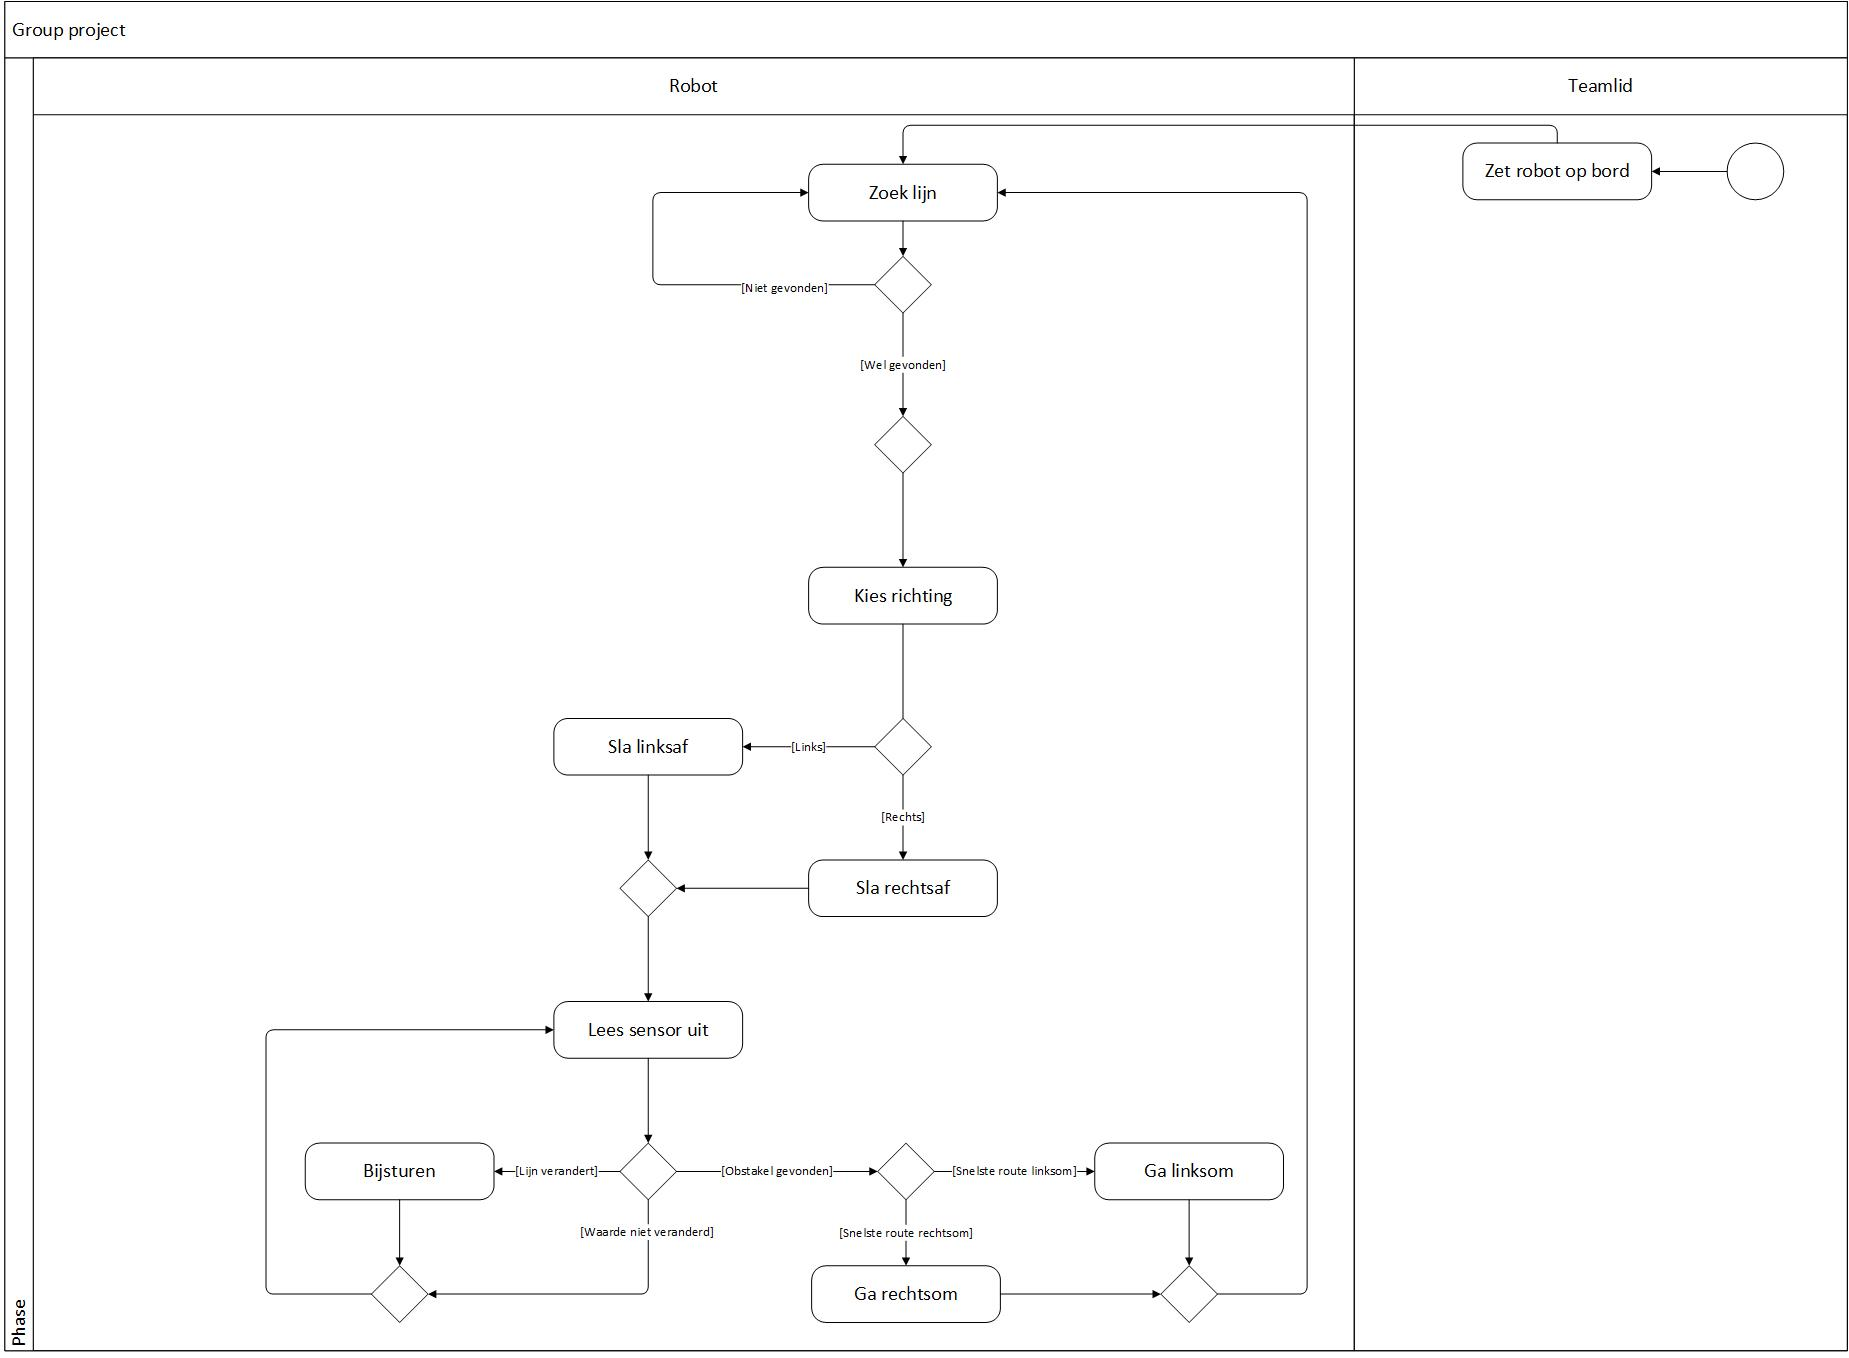
\includegraphics[scale=.4]{ActivityDiagramParcours1}
					\caption{Activity Diagram parcours 1}
				\end{SCfigure}
			\end{center}
			In deze figuur wordt er door middel van een Activity Diagram beschreven in wat voor status de robot zich kan bevinden in het eerste parcours, met eventueel een obstakel.
\newpage
		\subsubsection{Matrix}
			\begin{center}
				\begin{SCfigure}[0][h]
					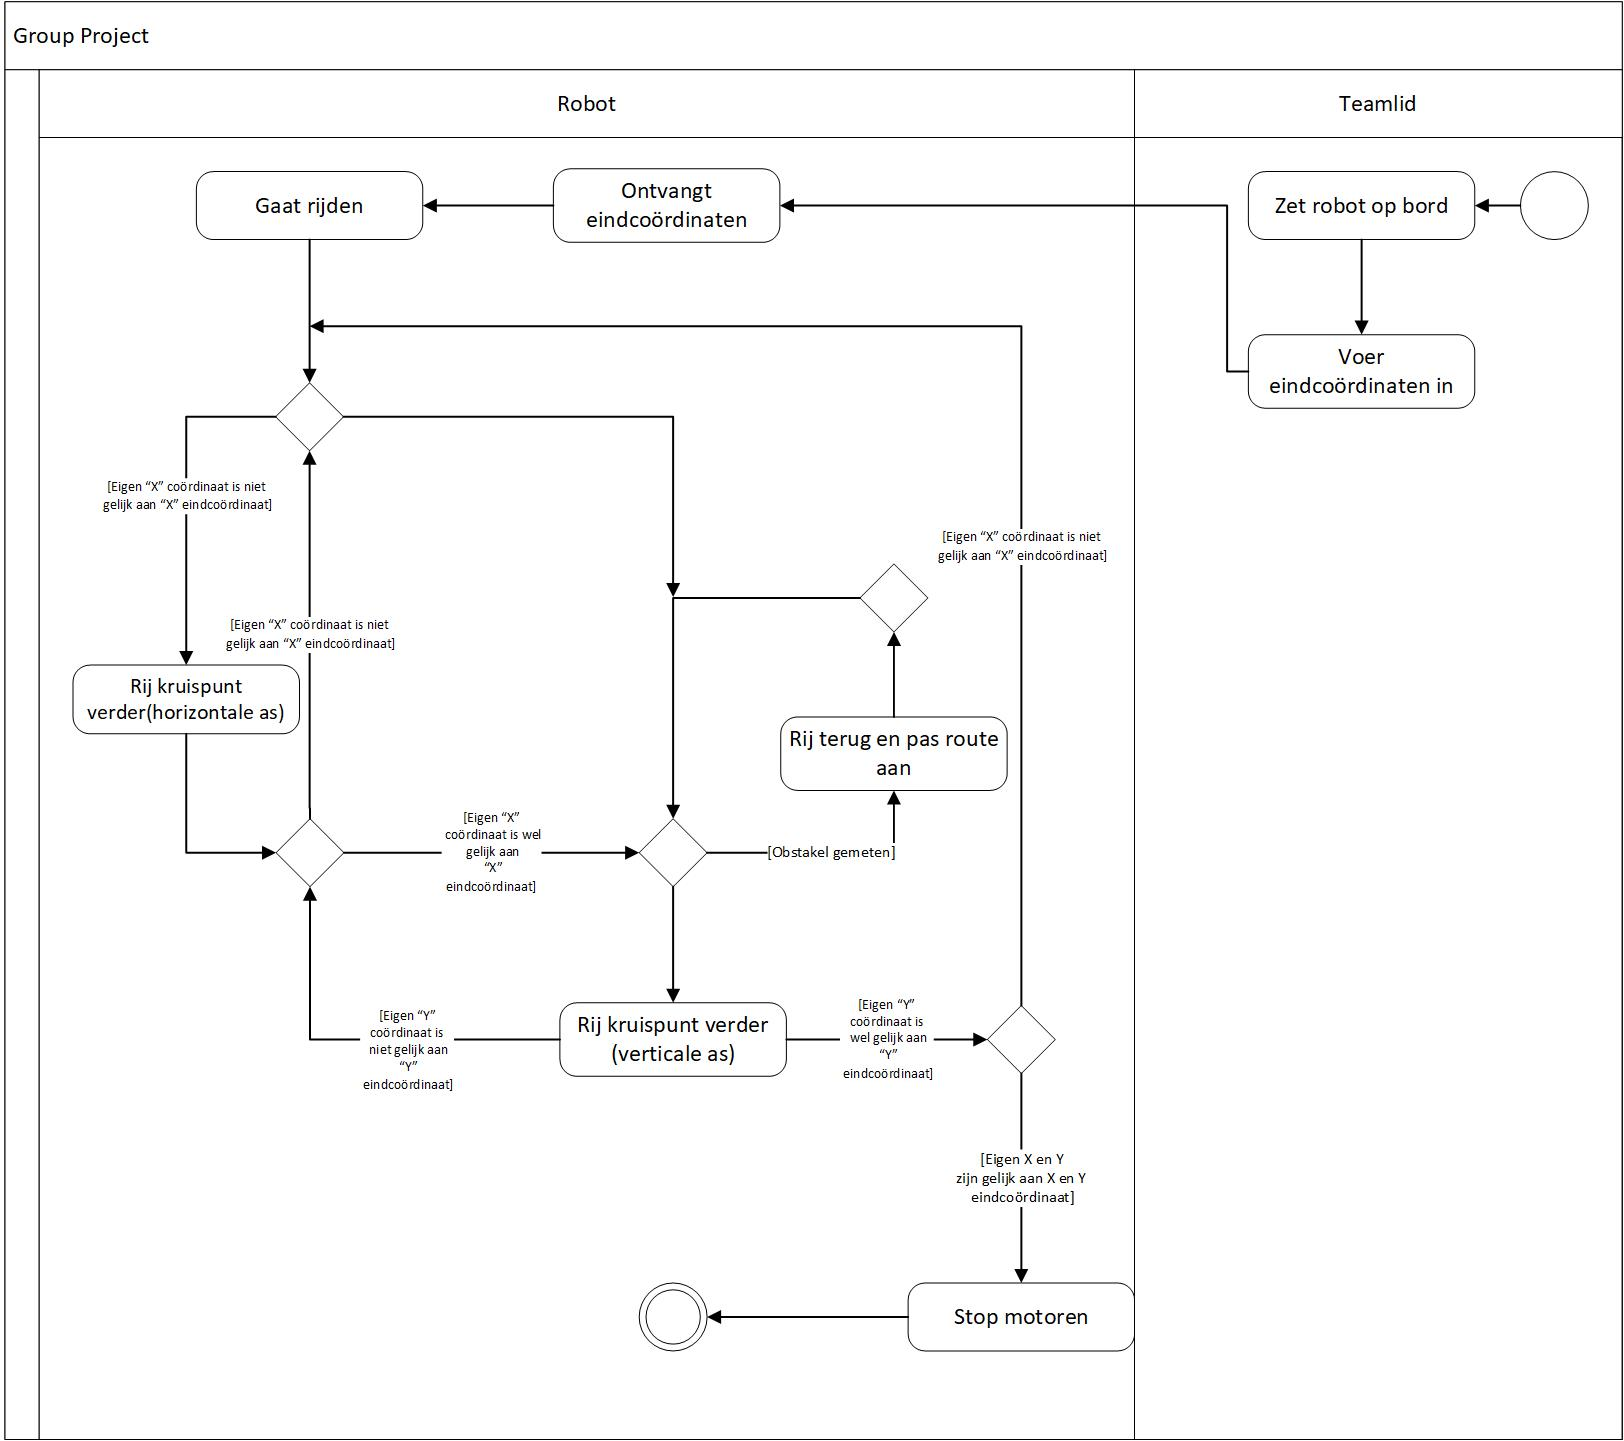
\includegraphics[scale=.5]{ActivityDiagramMatrix}
					\caption{Activity Diagram matrix parcours}
				\end{SCfigure}
			\end{center}
			In deze figuur wordt er door middel van een Activity Diagram beschreven in wat voor status de robot zich kan bevinden.
		\newpage
\section{Resultaten}
	In deze sectie zullen we de door ons ontwikkelde resultaten bespreken en visualiseren.
	\subsection{Motoren}
	De motoren zijn een belangrijk onderdeel van de robot. De motoren zorgen voor bochten, maar ook voor de snelheid voorwaarts. In deze paragraaf zullen we kort de werking beschrijven.
		\subsubsection{Sturing}
			Het maken van bochten wordt proportioneel gedaan. We kunnen de lichtwaardes meten en kijken wat wit, zwart en gecombineerd wit/zwart is. De x in onderstaande tabel is een gemeten waarde. De bevindingen zijn als volgt:
			%Tabel
			\begin{center}
				\begin{tabular}{ | p{3cm} | p{2cm}| p{2cm} | }
					\hline
					\multicolumn{3}{|c|}{ \textbf{Sensor waardes} } \\
					\hline
					& \textbf{Donker} & \textbf{Licht} \\ 
					\hline
					\textbf{Licht sensor} & \texttt{ x > 2000 } & \texttt{ x < 2000 } \\ 
					\hline
					\textbf{RGB sensor} & \texttt{ x < 450 } & \texttt{ x > 450 } \\ 
					\hline
				\end{tabular}
			\end{center}
		De volgende formule is gebruikt voor het proportioneel bijsturen van de motoren in de bochten:
		\begin{center}
			\Large $turn = K_{p} \times error$
		\end{center}
		Hierbij is $turn$ de bocht, $K_{p}$ de proportionele constante en $error$ de afwijking ten opzichte van de lijn.
		Je normaliseert de uitgelezen waarde van een sensor door de waarde af te trekken van de waarde die je wilt. Hierdoor krijg je een error.\newpage Negatief betekent van de lijn af sturen en positief betekent naar de lijn toe sturen. Zie hieronder voor een voorbeeld:
		\begin{center}
			\begin{SCfigure}[0.5][h]
				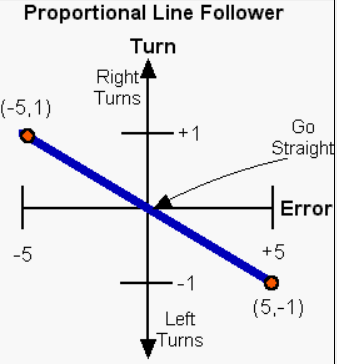
\includegraphics[scale=0.7]{proportional}
				\caption{Proportionele terugkoppeling}
			\end{SCfigure}
		\end{center}
\newpage
		\subsubsection{Code voorbeeld}
			Ook zullen we een heel klein eenvoudig stukje code bekijken die beide motoren laat draaien. Het autootje zal vooruit gaat bij het uitvoeren van deze functie.
			\begin{lstlisting}
				#include "motor_control.hpp"
				#include "BrickPi3.h"
				#include <stdio.h>
				#include <unistd.h>
				
				BrickPi3 MyBP; // new instance of BrickPi3 class
				int debug_motor = 0;
				
				void run_motor(int left_power, int right_power)
				{
				    MyBP.set_motor_power(PORT_C, right_power);
				    MyBP.set_motor_power(PORT_B, left_power);
				}
			\end{lstlisting}
			Bij de functie \texttt{void run\_motor(int left\_power, int right\_power)} zal er bij een gegeven \texttt{int left\_power} en \texttt{int right\_power} een afstand worden afgelegd.
		
		
	\subsection{Sensoren}
		Er worden twee sensoren gebruikt voor het meten van de zwart wit waardes zoals te zien in bovenstaande tabel. Tot slot is er nog een sensor voor het meten van een object.
		
		\subsubsection{RGB}
			Een RGB (Rood Groen Blauw) sensor, is een sensor die de drie zojuist genoemde kleuren projecteerd op een oppervlak. De sensor meet vervolgens de gereflecteerde kleuren en meet hieruit wat de waarde is. In dit project gebruiken wij alleen het rode licht. Het is namelijk in te stellen welk van de drie lichten je wilt gebruiken. Hierbij mag het voorzich spreken dat de waardes ook anders zijn als je dus andere lichten op een oppervlak projecteerd. Uiteraard is hier rekening mee gehouden.
			
		\subsubsection{Lichtsensor}
			Een lichtsensor meet de intensiteit van licht. Omdat zwart, licht absorbeert en wit, licht reflecteerd, is hieruit op te maken hoe licht of donker een bepaald oppervlak is. De waarde wordt hoger naarmate een oppervlak donkerder wordt en hoger als een oppervlak lichter wordt.
			
		\subsubsection{Ultrasoonsensor}
			Tot slot is er nog de ultrasoon sensor. Deze sensor meet aan de hand van een uitgezonden geluidssignaal de afstand tussen een potentieel object en zichzelf. Hiermee kunnen we een object dus herkennen. De volgende formule speelt hierbij een rol:
			\begin{center}
				\Large $v_{geluid} = 340\ m/s$ \\
				\Large $s_{lengte} = v_{geluid} \times (t / 2)$ \\[0.5cm]
			\end{center}
			Hieronder zullen we een kort stukje pseudocode beschrijven van het ontwijken van een object in een normaal parcours.
			\begin{lstlisting}
				int pre_defined_value = 10 // set the value to 10 cm
				while (true)
				{
				    if (ultrasonic_sensor > pre_defined_value)
				    {
					    dodge_cyclus(); // function to dodge the object
				    }
				}
			\end{lstlisting}
\newpage
\section{Conclusie}
	In dit kader bespreken we globaal de conclusies.
	\subsection{Parcours 1}
		De robot is in staat om soepel een lijn te volgen door middel van het proportionele algoritme. Ook kan de robot een obstakel ontwijken, als hij deze op de lijn tegenkomt. Tevens kan hij de lijn terugvinden.
	\subsection{Matrix}
		De robot is in staat een naar variable positie te navigeren. Elk kruispunt kan de robot herkennen. Mocht er een obstakel op de route zijn. Past de robot zijn route aan.
	\subsection{Eindconclusie}
		We kunnen hieruit concluderen dat de robot voldoet aan de gestelde eisen genoemd in sectie 2; Probleemstelling.
\end{document}